\subsubsection{Нет 2}
 
\zadatak Нађи вредности које задовољавају неједначину
\begin{align*}
\log_7 (x + 5) &> \log_5 (x + 5).
\intertext{\resenje Пребацимо израз у заједнички логаритам}
\frac{\log(x+5)}{\log7} &> \frac{\log(x+5)}{\log5} \\
\log5\log(x+5) &> \log7\log(x+5).
\intertext{Како је $\log5<\log7$ и позитивни су, да би услов важио, мора бити}
\log(x+5)&<0,
\intertext{одакле је}
x+5&<1\\
x&<-4,
\intertext{а да би логаритам био дефинисан мора да важи и}
x+5&>0\\
x&>-5,
\end{align*}
одакле је решење
$$
x\in\ram{(-5 ,-4)}.
$$
$$
\slika{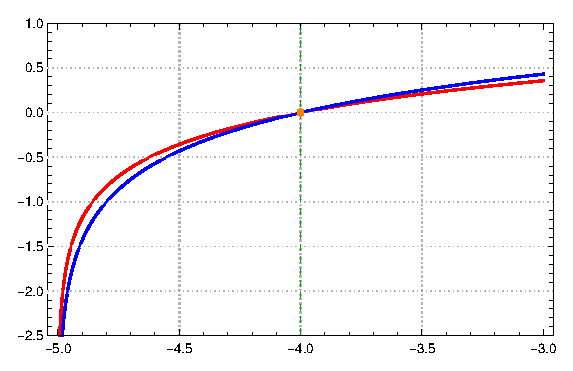
\includegraphics[width=\sirina]{eps/net2.eps}}{$y={\color{red}\log_7 (x + 5)};\, {\color{blue}\log_5 (x + 5)}$.}
$$
